\documentclass[11pt]{article}
\usepackage[T1]{fontenc}
\usepackage[margin=0.78in]{geometry}
\usepackage{amsmath,amssymb,amsthm}
\usepackage{graphicx}
\usepackage[hidelinks]{hyperref}
\usepackage{enumitem}

\newtheorem{theorem}{Theorem}
\newtheorem{corollary}[theorem]{Corollary}
\newcommand{\Z}{\mathbb Z}
\newcommand{\R}{\mathbb R}
\newcommand{\N}{\mathbb N}
\newcommand{\one}{\mathbf 1}
\newcommand{\Qbox}[1]{Q_{#1}}

\title{The diagonal sampled second-order Riesz transform is unbounded\\
\large A counterexample to Conjecture 1.4 of arXiv:2504.18739}
\author{Candidate counterexample packet}
\date{11 August 2026}

\begin{document}
\maketitle

\noindent\texttt{Status: counterexample\_likely\_valid.}

\section{Exact target}

Bañuelos and Kim define, for $d\geq2$ and $1<p<\infty$, the sampled
second-order transforms on $\ell^p(\Z^d)$ by
\begin{equation}\label{eq:def}
 R_{\mathrm{dis}}^{(jk)}f(n)
 =\sum_{m\in\Z^d}K_{\mathrm{dis}}^{(jk)}(m)f(n-m),\qquad
 K_{\mathrm{dis}}^{(jk)}(m)
 =c_d\frac{m_jm_k}{|m|^{d+2}}\one_{\Z^d\setminus\{0\}}(m),
\end{equation}
where $c_d=\pi^{-d/2}\Gamma((d+2)/2)>0$ \cite[(1.16)--(1.17)]{BK}.
The definition is reproduced verbatim below.

\begin{center}
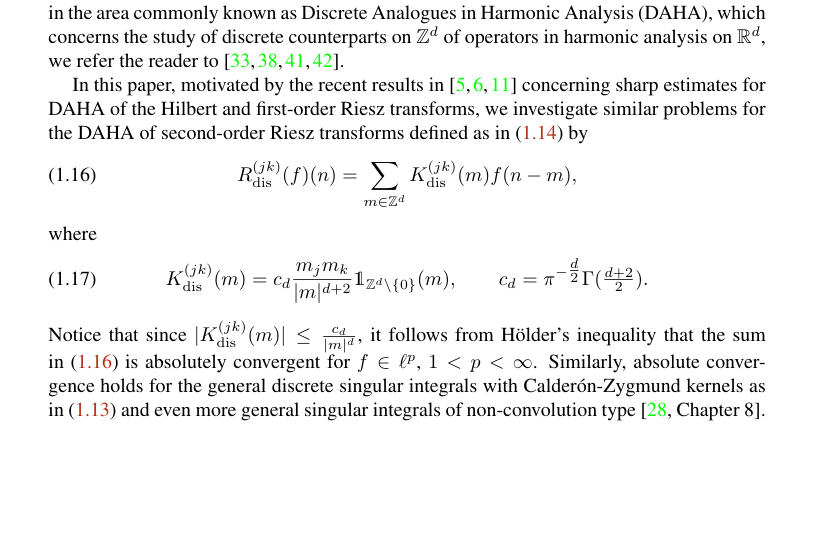
\includegraphics[width=.88\textwidth]{figures/source_definition.png}
\end{center}

Conjecture 1.4 then asserts, among other statements, that for every diagonal
index $j$,
\begin{equation}\label{eq:conj}
 \|\mathcal R^{(jj)}\|_{\ell^p\to\ell^p}
 =\|R_{\mathrm{dis}}^{(jj)}\|_{\ell^p\to\ell^p}
 =\|R^{(jj)}\|_{L^p\to L^p}.
\end{equation}

\begin{center}

\includegraphics[width=.88\textwidth]{figures/source_conjecture.png}
\end{center}

The diagonal sampled kernel in \eqref{eq:def} is nonnegative and has no
cancellation.  The next theorem shows that its norm is not merely larger than
the conjectured value: it is infinite.

\section{Counterexample theorem}

For $N\in\N$, write
\[
 \Qbox N=[-N,N]^d\cap\Z^d.
\]

\begin{theorem}\label{thm:main}
Fix $d\geq2$ and $j\in\{1,\dots,d\}$.  The convolution operator on finitely
supported sequences with kernel
\[
 k_j(m)=c_d\frac{m_j^2}{|m|^{d+2}}\one_{\Z^d\setminus\{0\}}(m)
\]
has no bounded extension to $\ell^p(\Z^d)$ for any $1<p\leq\infty$.
Consequently the diagonal assertion \eqref{eq:conj}, and hence Conjecture 1.4
as stated, is false.  Already for $p=2$,
\[
 \|R_{\mathrm{dis}}^{(jj)}\|_{\ell^2\to\ell^2}=\infty
 \quad\hbox{while}\quad
 \|R^{(jj)}\|_{L^2\to L^2}=\gamma(2)=1.
\]
\end{theorem}

\begin{proof}
Put
\[
 a_d=c_d(d+3)^{-(d+2)/2}>0.
\]
For an integer $L\geq1$, set $N=2^{L+1}$ and
$f_N=\one_{\Qbox{2N}}$.  For $q=0,\dots,L-1$, let $r_q=2^q$ and define the
disjoint lattice sets
\[
 S_q=\left\{m\in\Z^d:
 r_q\leq m_j<2r_q,\quad 0\leq m_i<r_q\ (i\neq j)\right\}.
\]
They satisfy $|S_q|=r_q^d$ and $S_q\subseteq\Qbox{N/2}$.  If $m\in S_q$,
then
\[
 m_j^2\geq r_q^2,
 \qquad
 |m|^2\leq \bigl(4+d-1\bigr)r_q^2=(d+3)r_q^2,
\]
and therefore
\begin{equation}\label{eq:shell}
 k_j(m)\geq a_d r_q^{-d}.
\end{equation}

Fix $n\in\Qbox N$.  For $m\in S_q\subseteq\Qbox{N/2}$ we have
$n-m\in\Qbox{3N/2}\subseteq\Qbox{2N}$, so $f_N(n-m)=1$.  Positivity of
$k_j$, disjointness of the $S_q$, and \eqref{eq:shell} give
\[
 (R_{\mathrm{dis}}^{(jj)}f_N)(n)
 \geq \sum_{q=0}^{L-1}\sum_{m\in S_q}k_j(m)
 \geq \sum_{q=0}^{L-1}r_q^d a_d r_q^{-d}
 =a_dL.
\]
Thus, for $1<p<\infty$,
\begin{align*}
 \frac{\|R_{\mathrm{dis}}^{(jj)}f_N\|_{\ell^p}}
      {\|f_N\|_{\ell^p}}
 &\geq a_dL\left(\frac{|\Qbox N|}{|\Qbox{2N}|}\right)^{1/p}\\
 &=a_dL\left(\frac{2N+1}{4N+1}\right)^{d/p}
 \geq a_d2^{-d/p}L\longrightarrow\infty.
\end{align*}
For $p=\infty$, the same pointwise estimate gives a ratio at least $a_dL$.
This proves unboundedness.  The last claim follows from the finite classical
norm recorded in \cite[(1.9), (1.24)]{BK}, with $\gamma(2)=1$.
\end{proof}

\section{Why the literal definition leaves no summation escape}

The test above uses only finitely supported $f_N$.  At every $n$, the sum in
\eqref{eq:def} then contains only finitely many nonzero terms.  Hence no
choice of principal value, enumeration, or convergence convention can alter
the estimate.  Adding a compensating local term or replacing $f(n-m)$ by
$f(n-m)-f(n)$ would define a different operator from (1.16)--(1.17).

The issue is the familiar cancellation obstruction for degree-$-d$ kernels.
For $j\neq k$, the angular factor $m_jm_k$ changes sign.  For the diagonal
sample it becomes $m_j^2\geq0$ and has positive mean on every fixed cone, so
each dyadic scale contributes a positive constant.  Classical diagonal
second-order Riesz transforms are distributional singular integrals with a
local compensation; simply deleting the origin and sampling the positive
off-origin function loses that compensation.

\begin{corollary}\label{cor:internal}
Under the literal definitions of \cite{BK}, the diagonal instance of the
comparison (1.21), the diagonal bound (3.15), and the all-index identity
\[
 \mathcal R^{(jk)}+R_{\mathrm{dis}}^{(jk)}
 =\mathcal J^{(jk)}*
 \quad\text{with }\mathcal J^{(jk)}\in\ell^1
\]
cannot all be valid for $j=k$.
\end{corollary}

\begin{proof}
The paper's martingale construction bounds $\mathcal R^{(jj)}$ on $\ell^p$,
and convolution by an $\ell^1$ sequence is bounded on $\ell^p$.  The displayed
identity would therefore make $R_{\mathrm{dis}}^{(jj)}$ bounded, contradicting
Theorem~\ref{thm:main}.
\end{proof}

\section{Audit of the diagonal proof}

The counterexample is independent of the source proof, but that proof shows
where the diagonal clause entered.  On PDF page 20, the integral of a product
of two derivative factors is separated into the factor
\[
F_2(m_j,t)F_3(m_k,t)
\]
times the remaining coordinate factors.  That separation is available when
$j\neq k$.  When $j=k$, both derivatives live in the same coordinate, so
their product must remain inside one one-dimensional integral; the displayed
product counts that coordinate twice.

There is also a visible sign failure on PDF page 21: a strictly positive
integral of
\[
 \frac{P_t^{(1)}(x)P_t^{(1)}(x-m)}{\theta(x,t)}
\]
is displayed as its own negative after a change of variables, and is then
declared zero.  Since each factor is positive, that conclusion cannot hold.
The relevant source passage is reproduced below.

\begin{center}
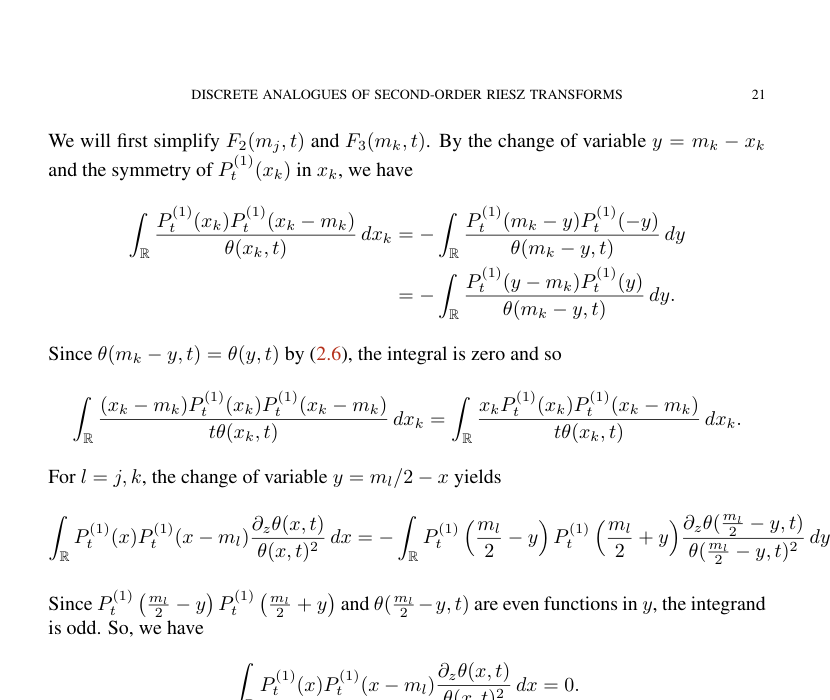
\includegraphics[width=.80\textwidth]{figures/source_proof_flaw.png}
\end{center}

Even if the latter line is treated as a typographical sign error, the
$j=k$ factorization failure and the direct box counterexample remain.

\section{Scope and upgrade audit}

The result is a full counterexample to Conjecture 1.4 because the conjecture
is a conjunction containing the universal diagonal clause (1.24).  The proof
strengthens the minimal $d=2$, $p=2$ refutation to every $d\geq2$, every
diagonal index, and every $1<p\leq\infty$.  At $p=1$, the image of a point
mass already fails to lie in $\ell^1$, since the positive kernel has divergent
total mass.

This packet does \emph{not} settle the off-diagonal equality (1.22), the
trace-free diagonal-difference equality (1.23), or the Beurling--Ahlfors
conjecture.  Those kernels retain cancellation and are not touched by the
positive-cone argument.  A natural repair is to restrict the sampled-kernel
program to off-diagonal and trace-free combinations, or to define a genuinely
compensated diagonal discretization.

Eight focused checks were made: literal source scope; the minimal
$d=2,p=2$ test; extension across $p$; extension across $d$; endpoint behavior;
the bounded-plus-$\ell^1$ consistency contradiction; localization of the
source proof failure; and bounded novelty/surviving-scope searches.  Searches
of the run's four lightweight indexes and by arXiv id, exact title, conjecture
number, and kernel formula found no correction, erratum, or prior
counterexample.  This is therefore a candidate result awaiting expert review,
not a definitive priority claim.

\section*{Human-review recommendation}

Check first that equations (1.16)--(1.17) are being read literally and that no
unwritten compensation convention is intended for $j=k$.  Under the displayed
definition, the dyadic-box proof is elementary and decisive.  A reviewer
should then compare the $j=k$ case against the published authors' intended
operator and decide whether the correct response is a counterexample to
(1.24) or an erratum to the diagonal definition.

\begin{thebibliography}{9}
\bibitem{BK}
R. Bañuelos and D. Kim,
\emph{Discrete analogues of second-order Riesz transforms},
arXiv:2504.18739v2 (2026); Conjecture 1.4.
\end{thebibliography}

\end{document}
